\documentclass[12pt,a4paper]{report}
\usepackage{amssymb,amsthm,amsmath,amscd}
\usepackage{latexsym}
\usepackage{enumerate}
\usepackage[german]{babel}
\usepackage{verbatim}
\usepackage[hyphens]{url}
\usepackage{hyperref}
\usepackage[utf8]{inputenc}
\usepackage{pdfpages}
\usepackage{graphicx}
\usepackage{csquotes}
\usepackage[landscape]{geometry}
\begin{document}
\begin{titlepage}
	\begin{center}

		\vspace*{1.0cm}
		\huge
		\textsc{\bf{PS Algorithmen für verteilte Systeme}}

		\vspace*{4.0cm}
		\textsc{
			\normalsize{eingereicht von} \\[0.5\baselineskip]
			{\large Baumgartner Dominik, Dafir Samy}
		}

		\vspace*{3.0cm}
		\textsc{
			\normalsize{Gruppe  1(16:00)}
		}

	\end{center}
\end{titlepage}

\section*{Aufgabe 15}
Im Folgenden sind die Knotengradverteilungen (Anzahl Knoten pro Knotengrad) für einen preferential attachment Graphen angeführt. Es wurden 3 Läufe ausgewertet.
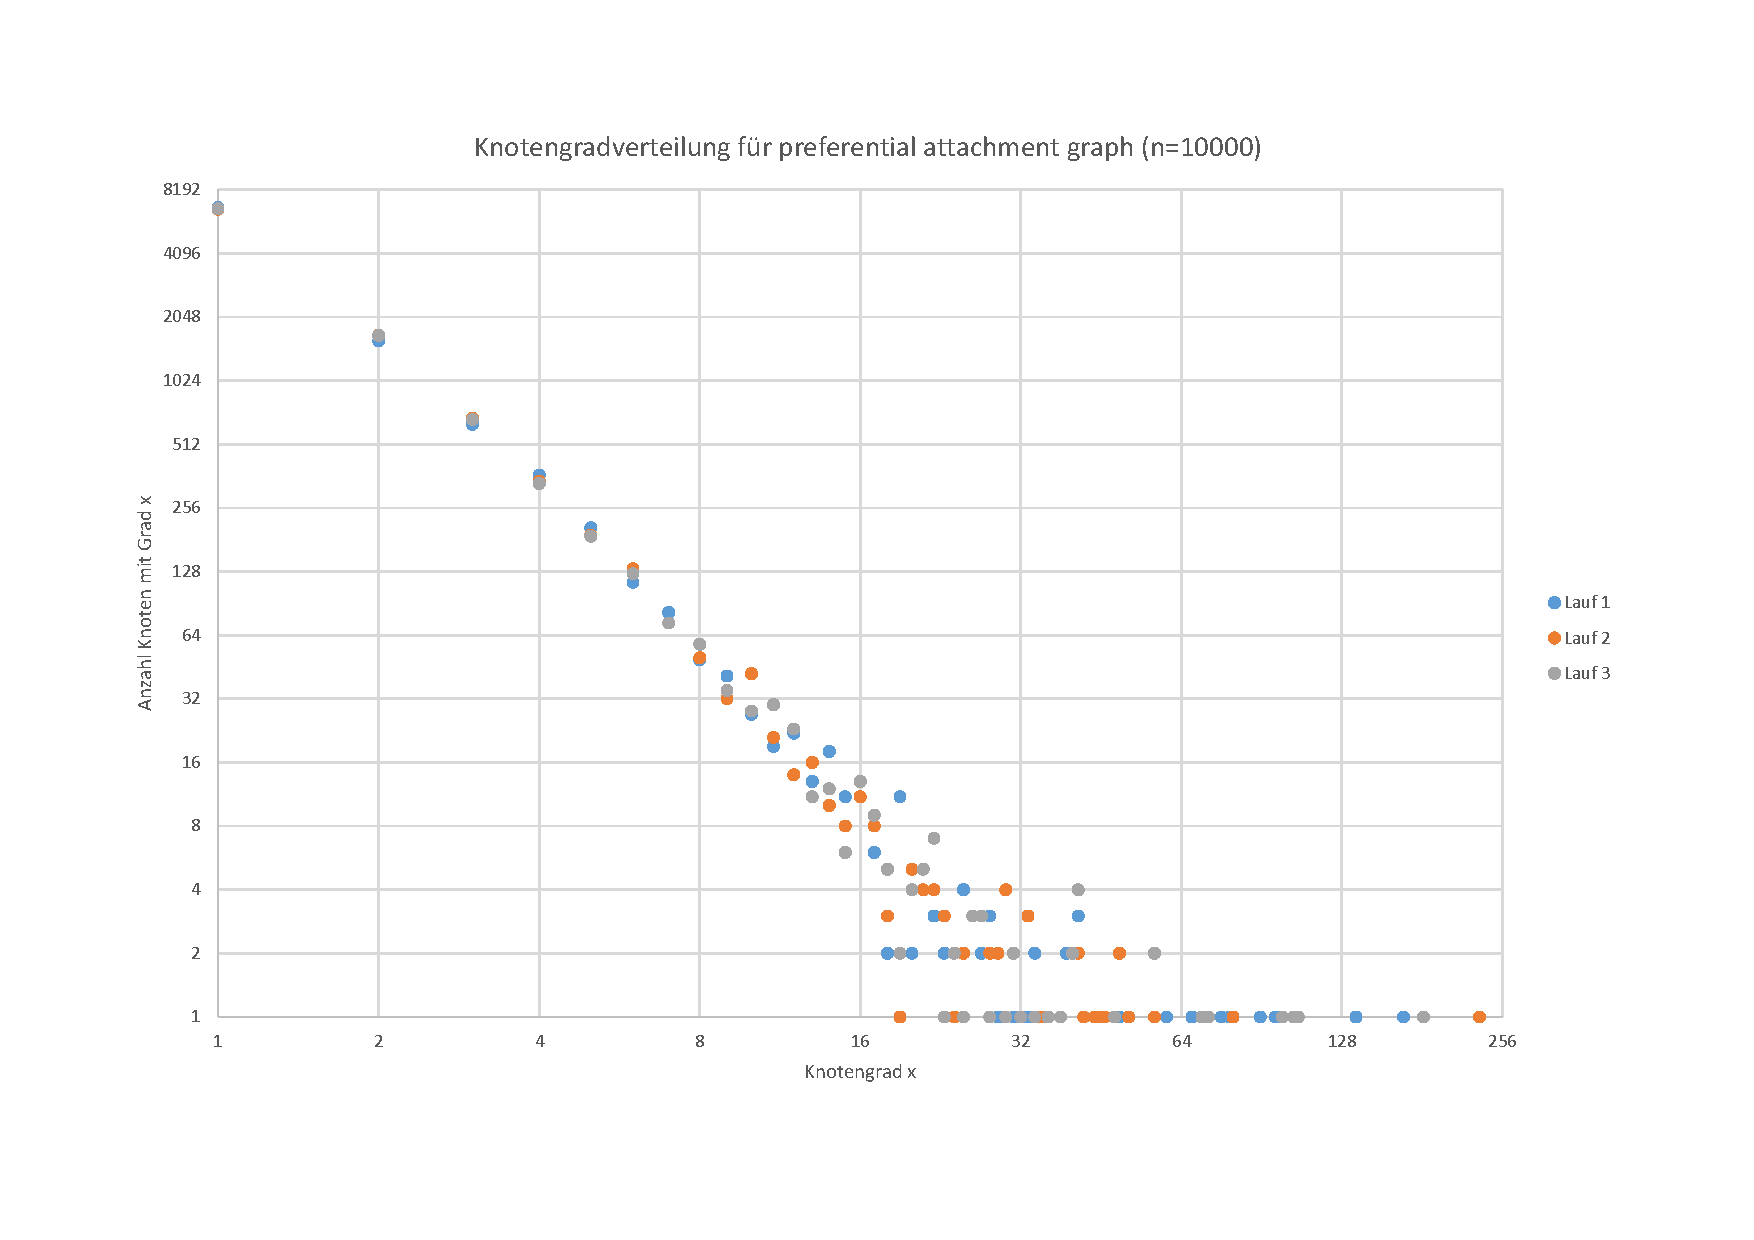
\includepdf[pages=-]{pagraph.pdf}
\end{document}
